\scanpage{54}
% archive sheet number: 53

\uline{\unsure{Réécrit|Récrit}} sans utiliser la partition des arcs critiques, pour déterminer les signes \deleted{de} $\varepsilon_{F'}(\deleted{\unsure{F}}a')$, quand on connaît \deleted{les $x'$ de} \inserted{les signes} $\varepsilon_F(a)$.

\uline{Proposition} \deleted{Considérons l'ens \deleted{\illegible{1}} $V_F$ (``verts'') des sommets d'ordre 4 incidents à $F$, et l'ens $\sigma_a^{F'}(V_{F'})$ (où $F'$ est la face incidente à $F$ le long de la grande arête $a$ de $\partial F$). \deleted{Soit \illegible{1}} Ces deux deux décomp\unsure{ositions|.} en arêtes de $\partial F$ ne \deleted{\unsure{que des}} \deleted{\unsure{ont, considérons}} \inserted{arêtes} considérons les (fermées) $\alpha$,}

Soit $A_{F,a}=$ \deleted{$A$} la réunion des grandes arêtes \inserted{$\alpha$} sur $F$ qui sont telles que $\sigma_a(\unsure{\alpha|a})$ soit une grande arête de $F'=\sigma_a(F)$ \unsure{à|a} (NB $a$ est une grande arête de $F$) Alors

a) $A$ est un arc sur $\partial F$, soit $B$ l'arc ``complémentaire''. \deleted{Alors} Considérons la subdivision de $B$ en grandes arêtes (sommets verts clairs) et en ``grandes arêtes pour $F'$'' (sommets verts foncés). Alors le nb d'arêtes $n_a(F)$ et $n_a(F')$ qui interviennent est \deleted{\unsure{ég}} compris entre 3 et 5 --- les possibilités sont (modulo échange de $F$ et $F'$) $(3,2),(3,3),(3,4)$ \deleted{Dans le} \deleted{\unsure{cas}} (cas 1) 2) 3)) --- et dans tous les cas, c'est la face spéciale qui donne lieu à 3 arcs (ce qui suffit à la déterminer, quand on est dans le cas $1^\circ$ ou $3^\circ$). De plus, on a

b) Si $\alpha$ est une \deleted{petite} arête \deleted{de} $F$ dans $A$, \deleted{\unsure{alors|al}} \deleted{alors} et $\alpha\ne a$, on a $\varepsilon_{F'}(a)=\varepsilon_F(a)$

[NB si $\alpha=a$, on a $\varepsilon_{F'}(a)=-\varepsilon_F(a)$]

c) On a les \deleted{\unsure{poss}} trois cas suivants \deleted{\unsure{fig}} pour la distribution des grandes arêtes sur $B$ (à échange près de $F$ et $F'$) et les signes correspondants

\deleted{\figure{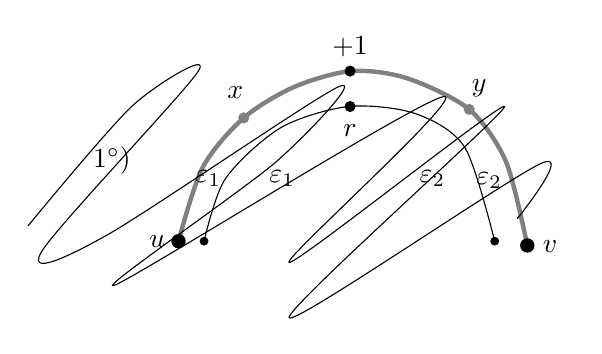
\begin{tikzpicture}[x=0.018cm,y=-0.018cm,line cap=round,line join=round]
\draw[gray,line width=1.6pt] plot[smooth] coordinates {(0,135) (17,83) (46,48) (82,26) (122,15) (161,20) (205,42) (231,79) (246,138)};
\fill[black] (0,135) circle [radius=2.6pt];
\fill[black] (246,138) circle [radius=2.6pt];
\fill[gray] (46,48) circle [radius=2pt];
\fill[gray] (205,42) circle [radius=2pt];
\node at (-47,78) {$1^\circ)$};
\node at (-15,135) {$u$};
\node at (262,139) {$v$};
\node at (40,30) {$x$};
\node at (212,27) {$y$};
\draw[thin] plot[smooth] coordinates {(18,135) (33,91) (72,55) (120,40) (167,45) (202,69) (223,135)};
\fill[black] (18,135) circle [radius=1.6pt];
\fill[black] (223,135) circle [radius=1.6pt];
\node at (21,91) {$\varepsilon_1$};
\node at (219,92) {$\varepsilon_2$};
\node at (73,91) {$\varepsilon_1$};
\node at (179,91) {$\varepsilon_2$};
\fill[black] (121,40) circle [radius=2pt];
\fill[black] (121,15) circle [radius=2pt];
\node at (121,57) {$r$};
\node at (121,-2) {$+1$};
\draw[thin] plot[smooth] coordinates {(-106,124) (-32,39) (14,15) (-97,143) (-51,131) (113,26) (70,78) (-45,166) (187,33) (78,150) (230,40) (78,189) (256,80) (239,119)};
\end{tikzpicture}}}

\deleted{\figure{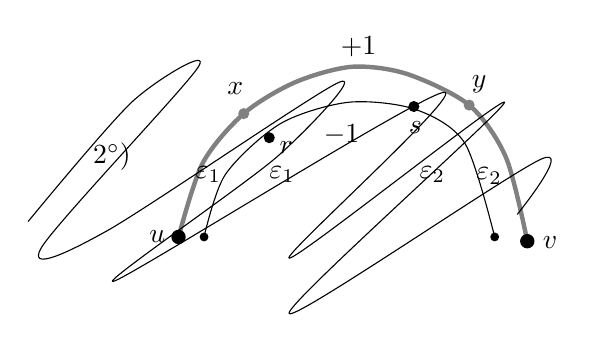
\begin{tikzpicture}[x=0.018cm,y=-0.018cm,line cap=round,line join=round]
\draw[gray,line width=1.6pt] plot[smooth] coordinates {(0,135) (17,83) (46,48) (82,26) (122,15) (161,20) (205,42) (231,79) (246,138)};
\fill[black] (0,135) circle [radius=2.6pt];
\fill[black] (246,138) circle [radius=2.6pt];
\fill[gray] (46,48) circle [radius=2pt];
\fill[gray] (205,42) circle [radius=2pt];
\node at (-47,78) {$2^\circ)$};
\node at (-15,135) {$u$};
\node at (262,139) {$v$};
\node at (40,30) {$x$};
\node at (212,27) {$y$};
\draw[thin] plot[smooth] coordinates {(18,135) (33,91) (72,55) (120,40) (167,45) (202,69) (223,135)};
\fill[black] (18,135) circle [radius=1.6pt];
\fill[black] (223,135) circle [radius=1.6pt];
\node at (21,91) {$\varepsilon_1$};
\node at (219,92) {$\varepsilon_2$};
\node at (73,91) {$\varepsilon_1$};
\node at (179,91) {$\varepsilon_2$};
\fill[black] (64,65) circle [radius=2pt];
\fill[black] (166,43) circle [radius=2pt];
\node at (76,72) {$r$};
\node at (167,58) {$s$};
\node at (115,63) {$-1$};
\node at (127,1) {$+1$};
\draw[thin] plot[smooth] coordinates {(-106,124) (-32,39) (14,15) (-97,143) (-51,131) (113,26) (70,78) (-45,166) (187,33) (78,150) (230,40) (78,189) (256,80) (239,119)};
\end{tikzpicture}}}

\deleted{\figure{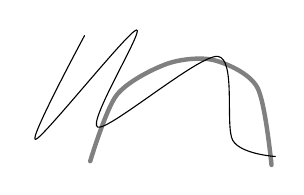
\begin{tikzpicture}[x=0.012cm,y=-0.012cm,line cap=round,line join=round]
\draw[gray,line width=1.6pt] plot[smooth] coordinates {(0,115) (28,45) (81,12) (131,8) (177,37) (192,119)};
\draw[thin] plot[smooth] coordinates {(-6,-18) (-58,92) (49,-24) (8,79) (135,4) (151,93) (196,110)};
\end{tikzpicture}}}

\figure{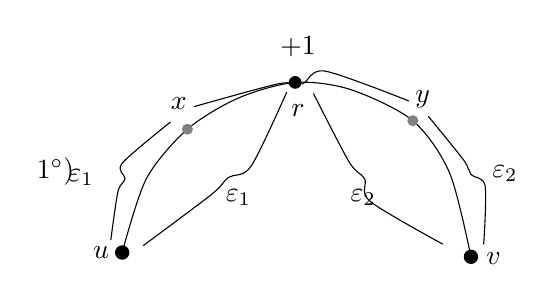
\begin{tikzpicture}[x=0.018cm,y=-0.018cm,line cap=round,line join=round]
\draw[thin] plot[smooth] coordinates {(0,135) (17,83) (46,48) (82,26) (122,15) (161,20) (205,42) (231,79) (246,138)};
\fill[black] (0,135) circle [radius=2.6pt];
\fill[black] (246,138) circle [radius=2.6pt];
\fill[gray] (46,48) circle [radius=2pt];
\fill[gray] (205,42) circle [radius=2pt];
\node at (-47,78) {$1^\circ)$};
\node at (-15,135) {$u$};
\node at (262,139) {$v$};
\node at (40,30) {$x$};
\node at (212,27) {$y$};
\draw[thin] plot[smooth] coordinates {(-8,126) (-3,92) (2,83) (0,72) (34,43)};
\node at (-29,82) {$\varepsilon_1$};
\draw[thin] plot[smooth] coordinates {(216,39) (241,70) (246,80) (256,88) (255,129)};
\node at (270,79) {$\varepsilon_2$};
\draw[thin] plot[smooth] coordinates {(51,32) (110,16) (127,16) (143,7) (202,28)};
\node at (124,-10) {$+1$};
\fill[black] (122,15) circle [radius=2.3pt];
\node at (124,35) {$r$};
\draw[thin] plot[smooth] coordinates {(15,130) (63,94) (75,82) (91,74) (116,22)};
\node at (82,96) {$\varepsilon_1$};
\draw[thin] plot[smooth] coordinates {(135,23) (160,71) (171,83) (175,99) (226,129)};
\node at (170,96) {$\varepsilon_2$};
\end{tikzpicture}}

\figure{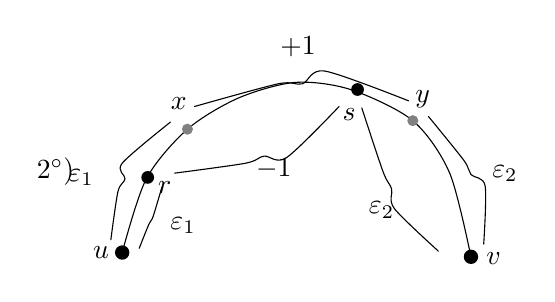
\begin{tikzpicture}[x=0.018cm,y=-0.018cm,line cap=round,line join=round]
\draw[thin] plot[smooth] coordinates {(0,135) (17,83) (46,48) (82,26) (122,15) (161,20) (205,42) (231,79) (246,138)};
\fill[black] (0,135) circle [radius=2.6pt];
\fill[black] (246,138) circle [radius=2.6pt];
\fill[gray] (46,48) circle [radius=2pt];
\fill[gray] (205,42) circle [radius=2pt];
\node at (-47,78) {$2^\circ)$};
\node at (-15,135) {$u$};
\node at (262,139) {$v$};
\node at (40,30) {$x$};
\node at (212,27) {$y$};
\draw[thin] plot[smooth] coordinates {(-8,126) (-3,92) (2,83) (0,72) (34,43)};
\node at (-29,82) {$\varepsilon_1$};
\draw[thin] plot[smooth] coordinates {(216,39) (241,70) (246,80) (256,88) (255,129)};
\node at (270,79) {$\varepsilon_2$};
\draw[thin] plot[smooth] coordinates {(51,32) (110,16) (127,16) (143,7) (202,28)};
\node at (124,-10) {$+1$};
\fill[black] (18,82) circle [radius=2.3pt];
\fill[black] (166,20) circle [radius=2.3pt];
\node at (30,89) {$r$};
\node at (160,38) {$s$};
\draw[thin] plot[smooth] coordinates {(12,132) (18,117) (20,113) (22,109) (28,89)};
\node at (43,116) {$\varepsilon_1$};
\draw[thin] plot[smooth] coordinates {(37,79) (87,72) (100,67) (116,68) (153,32)};
\node at (107,76) {$-1$};
\draw[thin] plot[smooth] coordinates {(169,33) (184,78) (190,90) (192,104) (223,134)};
\node at (183,105) {$\varepsilon_2$};
\end{tikzpicture}}

\figure{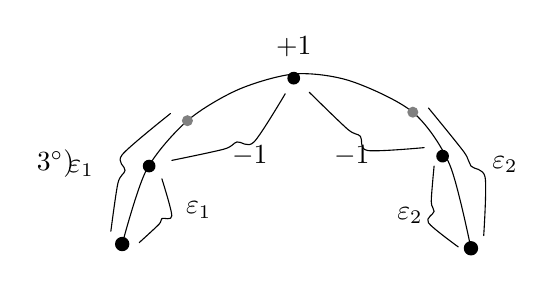
\begin{tikzpicture}[x=0.018cm,y=-0.018cm,line cap=round,line join=round]
\draw[thin] plot[smooth] coordinates {(0,135) (17,83) (46,48) (82,26) (122,15) (161,20) (205,42) (231,79) (246,138)};
\fill[black] (0,135) circle [radius=2.6pt];
\fill[black] (246,138) circle [radius=2.6pt];
\fill[gray] (46,48) circle [radius=2pt];
\fill[gray] (205,42) circle [radius=2pt];
\node at (-47,78) {$3^\circ)$};
\draw[thin] plot[smooth] coordinates {(-8,126) (-3,92) (2,83) (0,72) (34,43)};
\node at (-29,82) {$\varepsilon_1$};
\draw[thin] plot[smooth] coordinates {(216,39) (241,70) (246,80) (256,88) (255,129)};
\node at (270,79) {$\varepsilon_2$};
\fill[black] (19,80) circle [radius=2.3pt];
\fill[black] (121,18) circle [radius=2.3pt];
\fill[black] (226,73) circle [radius=2.3pt];
\node at (121,-4) {$+1$};
\draw[thin] plot[smooth] coordinates {(12,134) (26,121) (28,117) (35,115) (28,89)};
\node at (54,111) {$\varepsilon_1$};
\draw[thin] plot[smooth] coordinates {(35,76) (72,68) (81,63) (93,63) (115,29)};
\node at (90,73) {$-1$};
\draw[thin] plot[smooth] coordinates {(132,28) (159,54) (168,59) (173,69) (213,67)};
\node at (162,73) {$-1$};
\draw[thin] plot[smooth] coordinates {(220,80) (218,105) (220,112) (216,120) (237,137)};
\node at (203,115) {$\varepsilon_2$};
\end{tikzpicture}}
